\newpage 
\section[Continuity]{\hyperlink{toc}{Continuity}}

\subsection{Limits and Continuity}
\begin{definition}{Limits}{4.1}
    Let $X, Y$ be metric spaces. Let $E \subset X$, and let $f: E \mapsto Y$. Let $p \in X$ be a limit point of $E$. Then, we say that $\lim_{x\rightarrow p} f(x) = q$ or $f(x) \rightarrow q$ as $x \rightarrow p$ if there exists $q \in Y$ such that for all $\e > 0$, there exists $\delta > 0$ such that for all $x \in E$ with $0 < d_X(x, p) < \delta$ we have that $d_Y(f(x), q) < \e$. 
\end{definition}
\begin{figure}[htbp]
    \centering
    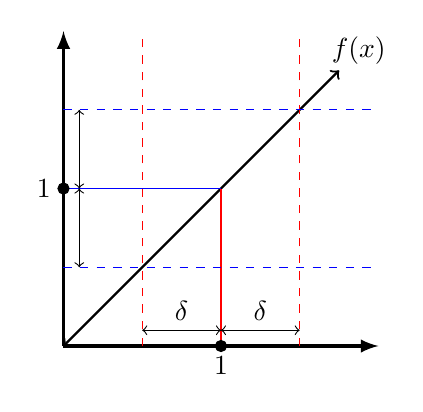
\begin{tikzpicture}[scale=2]
        \draw[-latex,very thick] (0,0)--(2,0);
        \draw[-latex,very thick] (0,0)--(0,2);
        \draw[<->, thick] (0, 0) -- (1.75, 1.75);
        \draw[color = red] (1, 0) -- (1, 1);
        \draw[color = red, dashed] (0.5, 0) -- (0.5, 2);
        \draw[color = red, dashed] (1.5, 0) -- (1.5, 2);
        \draw[<->] (0.5, 0.1) -- (1, 0.1);
        \node[above] at (0.75, 0.1) {$\delta$};
        \draw[<->] (1, 0.1) -- (1.5, 0.1);
        \node[above] at (1.25, 0.1) {$\delta$};
        \draw[color = blue] (0, 1) -- (1, 1);
        \draw[color = blue, dashed] (0, 0.5) -- (2, 0.5);
        \draw[color = blue, dashed] (0, 1.5) -- (2, 1.5);
        \draw[<->] (0.1, 0.5) -- (0.1, 1);
        \node[right] at (0.1, 0.75) {$\e$};
        \draw[<->] (0.1, 1) -- (0.1, 1.5);
        \node[right] at (0.1, 1.25) {$\e$};
        \draw[fill = black] (0, 1) circle (1pt);
        \node[xshift = -0.25cm] at (0, 1) {$1$};
        \draw[fill = black] (1, 0) circle (1pt);
        \node[yshift = -0.25cm] at (1, 0) {$1$};
        \node[yshift = 0.25cm, xshift = 0.25cm] at (1.75, 1.75) {$f(x)$};
    \end{tikzpicture}
    \caption{Visualization of the limit $\lim_{x \rightarrow 1}f(x) = 1$ for $f(x) = x$. For any $\e > 0$, we can take $\delta = \e$ and then we have that $\abs{f(x) - 1} < \e$ if $\abs{x - 1} < \delta$.}
    \label{fig17}
\end{figure}
Note in the above definition that we do not care about $f(p)$, that is, the actual value of $f$ at $p$. In particular, if $p \notin E$, then $f(p)$ is not even necessarily defined. This distinction between the limit and the actual value of a function at a point becomes crucial later on when we want to define a derivative. Although we will discuss this in more detail in Chapter 5, the definition of a derivative of a function $g$ at a point $p \in \RR$ involves the function $f: \RR \rightarrow \RR$ such that:
\begin{align*}
    f(x) = \frac{g(x) - g(p)}{x - p}
\end{align*}
Evidently, the domain of $f$ does not contain the point $p$, but we are interested in the value of $f$ in the limit of $x \rightarrow p$ (which, if it exists, is the value of the derivative).

\begin{figure}[htbp]
    \centering
    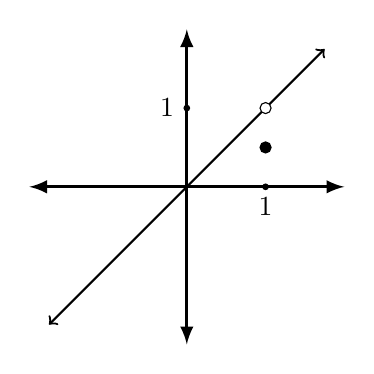
\begin{tikzpicture}
        \draw[latex-latex,very thick] (-2,0)--(2,0);
        \draw[latex-latex,very thick] (0,-2)--(0,2);
        \draw[<->, thick] (-1.75, -1.75) -- (1.75, 1.75);
        \draw[fill = black] (0, 1) circle (1pt);
        \node[xshift = -0.25cm] at (0, 1) {$1$};
        \draw[fill = black] (1, 0) circle (1pt);
        \node[yshift = -0.25cm] at (1, 0) {$1$};
        \draw[fill = white] (1, 1) circle (2pt);
        \draw[fill = black] (1, 0.5) circle (2pt);
    \end{tikzpicture}
    
    \caption{Visualization of the function $f(x) = x$ for $x \in \RR \setminus \set{1}$, $f(x) = 0$ for $x = 1$. In this case, we have that $f(1) = 0$ but $\lim_{x \rightarrow 1} f(x) = 1$, demonstrating that the actual value of the function is irrelevant when defining the limit.}
    \label{fig18}
\end{figure}

\begin{theorem}{}{4.2}
    Let $X, Y$ be metric spaces. Let $E \subset X$ and $f:E \mapsto Y$. Suppose that for all sequences $\set{p_n} \subset E$ with $p_n \rightarrow p$ and $p_n \neq p$, we have that $f(p_n) \rightarrow q \in Y$. Then, this is equivalent to saying that $\lim_{x \rightarrow p} f(x) = q$.
\end{theorem}
\begin{nproof}
    \boxed{\implies} Suppose that $\lim_{x \rightarrow p} f(x) = q$, and let $\set{p_n}$ be a sequence in $E$ with $p_n \rightarrow p$ and $p_n \neq p$ for all $n$. We wish to show that $f(p_n) \rightarrow q$. Let $\e > 0$. We show that there exists $N \in \NN$ such that $d_Y(f(p_n), q) < \e$ for all $n \geq N$. Since $\lim_{x \rightarrow p} f(x) = q$, there exists $\delta > 0$ such that for all $x \in E$ with $d_X(p, x) < \delta$, $d_Y(f(x),q) < \e$. Since we know that $p_n \rightarrow p$, there exists some $N$ such that $0 < d(p_n, p) < \delta$ for all $n \geq N$, so we have that $d_Y(f(p_n), q) < \e$ as required. 

    \boxed{\impliedby} We show the contrapositive. Suppose that $\lim_{x \rightarrow p} f(x) \neq q$. We wish to find a sequence $\set{p_n} \subset E$ with $p_n \rightarrow p$ and $p_n \neq p$ for all $n$ such that $f(p_n)$ does not converge to $q$. Since $\lim_{x \rightarrow p} f(x) \neq q$, then there exists $\e > 0$ such that for all $\delta > 0$, there exists $x \in E$ such that $0 < d_X(x, p) < \delta$ but $d_Y(f(x), q) \geq \e$. For each $\delta$ of the form $\frac{1}{n}$, let $p_n \in E$ be the corresponding value of $x$. Then, $p_n \rightarrow p$, $p_n \neq p$ for all $n$, and $f(p_n)$ does not converge to $q$ as $d(f(p_n), q) \geq \e$ for all $n$. \qed
\end{nproof}

\stepcounter{rudin}

\begin{theorem}{}{4.4}
    When $Y = \CC$ (i.e. the functions we consider are complex), then limits respect sums, differences, products, and functions. That is, let $X$ is a metric space, $E \subset X$, and $f, g: E \mapsto \CC$ with $p$ a limit point of $E$. If $\lim_{x \rightarrow p}f(x) = q$ and $\lim_{x \rightarrow p}g(x) = r$, then $\lim_{x \rightarrow p}(f+g)(x) = q + r$. The same holds for subtraction, multiplication, and division (provided we do not divide by zero).
\end{theorem}
\begin{nproof}
    By Theorem \ref{thm:4.2}, these properties of limits follow from the analogous properties of sequences (Theorem \ref{thm:3.3}).
\end{nproof}

\begin{definition}{Continuity}{4.5}
    Let $X, Y$ be metric spaces, and $E \subset X$. Let $p \in E$, and define $f: E \mapsto Y$. We say that $f$ is continuous at $p$ if for all $\e > 0$, there exists $\delta > 0$ such that for all $x \in E$ with $d_X(x, p) < \delta$, we have that $d_Y(f(x), f(p)) < \e$. Equivalently, $f(N_\delta^E(p)) \subset N_\e^Y(f(p))$. If $f$ is continuous at $p$ for all $p \in E$, we say that $f$ is continuous.
\end{definition}
\noindent Note that this definition of continuity is heavily reliant on the particular metric of $X$ and $Y$; in particular, there can be functions that are continuous for some choices of metric but not others.

Let us consider some examples of continuous functions (while thinking about different possible metric spaces). 

First, let us take onsider $X = E = \ZZ$ and $Y = \RR$. What functions $f: E \rightarrow Y$ are continuous at $p = 0$? The answer turns out to be all functions! To see this, fix $n \in \ZZ$ and let $\e > 0$. We then have that if $\abs{n - m} < \frac{1}{2}$, then $\abs{f(n) - f(m)} < \e$ as the only point $m$ contained in $N_{1/2}^\ZZ(n)$ is $n$ itself (and hence $\abs{f(n) - f(m)} = \abs{f(n) - f(n)} = 0$). This argument applies to every $n \in \ZZ$ and hence all functions $f: \ZZ \mapsto \RR$ are continuous.

As further examples (that work for arbitrary metric spaces), If we have that $f: X \mapsto X$, $f(x) = x$, we have that $f$ is continuous (pick $\delta = \e$ in the definition of continuity). If we have that $f: X \mapsto Y$, $f(x) = c$ for some $c \in Y$, then $f$ is also continuous (pick any $\delta > 0$ in the definition). 
 
We now consider a Theorem which gives us a familiar notion of continuity (that may have been encountered in first year calculus).

\begin{theorem}{}{4.6}
    Suppose that $p$ is a limit point of $E$ in Definition \ref{def:4.5}. Then, $f$ is continuous at $p$ if and only if $\lim_{x \rightarrow p}f(x) = f(p)$. 
\end{theorem}
\begin{nproof}
    The claim immediately follows by comparing Definitions \ref{def:4.1} and \ref{def:4.5}. \qed
\end{nproof}

\begin{theorem}{}{4.7}
    Let $X, Y, Z$ be metric spaces, and $E \subset X, F \subset Y$. Let $f: E \mapsto Y$, $g: F \mapsto Z$, and suppose $f(E) \subset F$. Let $p \in E$. If $f$ is continuous at $p$ and $g$ is continous at $f(p)$, then $g \circ f: E \mapsto Z$ is continuous at $p$.
\end{theorem}
\begin{nproof}
    Let $\e > 0$. Since $g$ is continuous at $f(p)$, there exists $\gamma > 0$ such that $d_Z(g(y), g(f(p))) < \e$ if $d_Y(y, f(p)) ,< \gamma$. Since $f$ is continuous at $p$, there exists $\delta > 0$ such that $d_Y(f(x), f(p)) < \gamma$ if $d_X(x, p) < \delta$. Hence, we have that $d_Z(h(x), h(p)) = d_Z(g(f(x)), g(f(p))) < \e$ if $d_X(x, p) < \delta$ and $x \in E$. We conclude that $h$ is continuous at $p$. \qed
\end{nproof}

\subsection{Topological Characterization of Continuity}

\subsection{Continuity and Compactness}

\subsection{Uniform Continuiity, Connectedness, and IVT}

